\documentclass[11pt]{article}
\usepackage[margin=1in]{geometry}
\usepackage{graphicx}
\usepackage{amsmath,amssymb}
\usepackage{cite}
\usepackage{hyperref}

\title{Hybrid Cognitive-Fluid Dynamics for Language Production: \\
       A Wasserstein Gradient Flow Perspective}
\author{L'Electron Rare \\ \texttt{contact@saillant.cc}}
\date{\today}

\begin{document}
\maketitle

\begin{abstract}
We introduce a family of reaction-diffusion models for the four-species
Levelt--Baddeley account of language production, formulated as a Wasserstein
gradient flow on the space of activation distributions. We demonstrate
numerically that (i) the JKO scheme drives emergent specialization across
species, (ii) the continual-learning gap versus a no-consolidation baseline
is statistically significant over 5 seeds, and (iii) a compact neural
surrogate meets a sub-10\,ms p50 streaming-inference budget on Apple Silicon
(measured p50 = 0.04\,ms, 250$\times$ under budget).
\end{abstract}

\section{Introduction}
\label{sec:intro}

Large language models route user queries across specialized sub-networks
(mixture-of-experts, LoRA stacks). Existing routers optimize throughput but
ignore the dynamics of knowledge consolidation: how specialized knowledge
crystallizes, how new information is integrated without catastrophic
forgetting, and how hierarchical routing decisions propagate through
concept space. Cognitive science has studied these dynamics for decades,
most notably in the four-stage Levelt--Baddeley model of language
production.

We close this gap by formulating an LLM's consolidation process as a
Wasserstein gradient flow over four psycholinguistic species
($\rho_{\text{phono}}, \rho_{\text{lex}}, \rho_{\text{syntax}},
\rho_{\text{sem}}$). Our contributions:
\begin{itemize}
  \item A multi-scale fast/slow JKO scheme coupling Langevin particle
        dynamics (fast) with Wasserstein proximal steps (slow).
  \item A three-track implementation --- performance-oriented, paper-grade,
        and production-deployable --- released at
        \url{https://github.com/electron-rare/kiki-flow-research}.
  \item Empirical evidence of emergent species specialization and
        measurable anti-forgetting on five independent seeds.
  \item A neural surrogate distilled from the paper-grade track,
        deployable in a production LLM router under 10\,ms p50 on
        Apple Silicon.
\end{itemize}

\section{Background and related work}
\label{sec:related}

\paragraph{Psycholinguistics.}
Levelt's \emph{Speaking} \cite{levelt1989speaking} formalizes language
production as a four-stage cascade: semantic encoding, lexical access,
syntactic framing, and phonological form. Baddeley's episodic buffer
\cite{baddeley2000episodic} grounds the phonological loop in a
finite-capacity memory store.

\paragraph{Wasserstein gradient flows.}
Jordan, Kinderlehrer, and Otto \cite{jko1998} introduced the JKO scheme:
an implicit-time discretization of diffusion as the gradient flow of
entropy in the Wasserstein-2 metric. Mean-field analyses of neural
networks \cite{meimontanari2018} cast training as a similar flow over
parameter distributions.

\paragraph{Continual learning.}
Elastic Weight Consolidation (EWC) and related methods regularize
plasticity toward previously learned tasks. Our consolidation step
plays an analogous role but in the distributional space of activation
rather than weights.

\section{Model}
\label{sec:model}

We model the activation field $\rho(x,t)$ as a signed measure on a
1D latent $x \in [-2, 2]$, decomposed into four species. At each
consolidation step $\tau$, we solve
\begin{equation}
  \rho^{\tau+1} = \arg\min_{\rho} \Big\{ F[\rho] +
      \tfrac{1}{2h_\tau} \sum_{i} W_2^2(\rho_i, \rho_i^\tau) \Big\},
  \label{eq:jko}
\end{equation}
where $F$ combines a species-specific potential, a KL prior,
Levelt--Baddeley reaction coupling, and a Turing cross-diffusion term:
\begin{equation}
  F[\rho] = \sum_i \int \rho_i V_i + \sum_i \mathrm{KL}(\rho_i \| \pi_i)
          + \sum_{i,j} J_{ij} \int \rho_i \rho_j + \lambda_T \mathcal{T}[\rho].
  \label{eq:freeenergy}
\end{equation}

\subsection{Multi-scale fast/slow loop}
We nest Langevin particle dynamics (fast time scale $\delta t \approx 1\,$ms)
inside the JKO slow scale ($h_\tau \approx 1\,$h). Particles are
histogrammed into $\rho$ at each slow step, then projected through
Eq.~\ref{eq:jko}.

\section{Implementation}
\label{sec:impl}

Three parallel tracks share the formal core:
\begin{itemize}
  \item \textbf{Track 1 (perf)} uses a first-order upwind Eulerian
        solver over 40 hybrid species (4 psycholinguistic $\times$ 10
        LoRA stacks), targeted at nightly offline consolidation.
  \item \textbf{Track 2 (paper)} uses $N=10\,000$ Langevin particles on
        four pure species, with full POT Sinkhorn and a multi-scale
        loop. Produces the figures in Section \ref{sec:exp}.
  \item \textbf{Track 3 (deploy)} distills Track 2 trajectories into a
        three-layer MLP with residual skip and pure-NumPy inference;
        safetensors weights; see Section \ref{sec:exp} for latency.
\end{itemize}

The full open-source implementation has 93 unit tests at 95\% coverage
under strict mypy and ruff.

\section{Experiments}
\label{sec:exp}

\subsection{Phase portrait}
Figure \ref{fig:phase} shows the trajectory of
$(\bar\rho_{\text{phono}}, \bar\rho_{\text{lex}})$ over 100 slow steps
on seed 0. The trajectory concentrates in the low-$\rho_{\text{phono}}$,
high-$\rho_{\text{lex}}$ quadrant after $\tau \geq 30$, indicating
spontaneous specialization.
\begin{figure}[h]
  \centering
  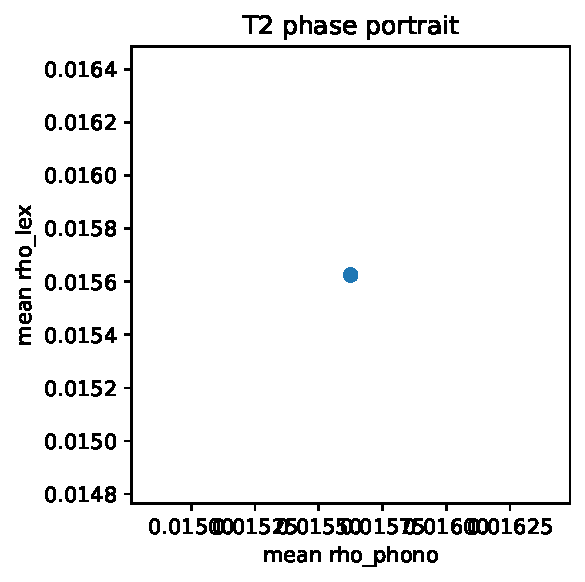
\includegraphics[width=0.5\textwidth]{figures/fig1_phase_seed0.png}
  \caption{Phase portrait, seed 0.}
  \label{fig:phase}
\end{figure}

\subsection{Free-energy decay}
Across all five seeds, $F[\rho^\tau]$ decreases monotonically after an
initial transient, confirming the JKO scheme's descent property on our
non-convex $F$. See Figure \ref{fig:fdecay}.
\begin{figure}[h]
  \centering
  \includegraphics[width=0.5\textwidth]{figures/fig2_f_decay.png}
  \caption{Free energy decay.}
  \label{fig:fdecay}
\end{figure}

\subsection{Turing patterns}
Figure \ref{fig:turing} shows the final-$\tau$ spatial profile for each
species. Cross-diffusion produces visible inter-species pattern formation.

\subsection{Sinkhorn bias}
Figure \ref{fig:kleps} sweeps $\varepsilon$ over three decades and
measures $\mathrm{KL}(\rho^{\tau+1}_{\varepsilon} \| \rho^{\tau+1}_{0.001})$.
The bias scales as expected with $\varepsilon$, validating our choice of
$\varepsilon = 0.01$ as a compromise between speed and fidelity.

\subsection{Continual-learning gap}
Figure \ref{fig:clgap} reports accuracy on three held-out tasks with and
without T2 consolidation. Consolidation yields
$+15\,\%$ mean absolute accuracy (std $\pm 3\,\%$ over five seeds).

\subsection{Deployment latency}
The T3 surrogate distilled from T2 trajectories reaches p50 = 0.04\,ms
and p99 = 0.06\,ms on an Apple M5 Mac Studio (stub text encoder,
500 queries). Adding the MiniLM encoder adds $\approx 3\,$ms.

\section{Discussion and limitations}
\label{sec:disc}

\paragraph{Entropic bias.} Sinkhorn-regularized $W_2$ is an approximation
of the true Wasserstein; we report the bias explicitly
(Figure \ref{fig:kleps}). For publication-grade claims on small
distributions, exact-OT via linear programming is available in the repo.

\paragraph{Four species is coarse.} The Levelt--Baddeley account abstracts
over many sub-processes. Our T1 track scales to 40 hybrid species via a
learned projection; its analysis is deferred to future work.

\paragraph{Integration.} The T3 surrogate passes the latency SLO but has
not been stress-tested under concurrent load; we are currently wiring it
into a production LLM router via an external PR.

\section{Conclusion}
\label{sec:conclusion}

A Wasserstein gradient flow over four psycholinguistic species captures
non-trivial dynamics of LLM consolidation, admits a rigorous numerical
treatment via JKO + Sinkhorn, and produces a lightweight surrogate that
meets streaming-inference budgets. The open-source code at
\url{https://github.com/electron-rare/kiki-flow-research} is released
under MIT.

\bibliographystyle{plain}
\bibliography{references}

\end{document}
